% This document has been modified from its original version by Kathryn Huff 
% Acknowledgement of the original version is below.
%
%%%%%%%%%%%%%%%%%%%%%%%%%%%%%%%%%%%%%%%%%
% Academic Title Page
% LaTeX Template
% Version 2.0 (17/7/17)
%
% This template was downloaded from:
% http://www.LaTeXTemplates.com
%
% Original author:
% WikiBooks (LaTeX - Title Creation) with modifications by:
% Vel (vel@latextemplates.com)
%
% License:
% CC BY-NC-SA 3.0 (http://creativecommons.org/licenses/by-nc-sa/3.0/)
% 
% Instructions for using this template:
% This title page is capable of being compiled as is. This is not useful for 
% including it in another document. To do this, you have two options: 
%
% 1) Copy/paste everything between \begin{document} and \end{document} 
% starting at \begin{titlepage} and paste this into another LaTeX file where you 
% want your title page.
% OR
% 2) Remove everything outside the \begin{titlepage} and \end{titlepage}, rename
% this file and move it to the same directory as the LaTeX file you wish to add it to. 
% Then add \input{./<new filename>.tex} to your LaTeX file where you want your
% title page.
%
%%%%%%%%%%%%%%%%%%%%%%%%%%%%%%%%%%%%%%%%%

%----------------------------------------------------------------------------------------
%    PACKAGES AND OTHER DOCUMENT CONFIGURATIONS
%----------------------------------------------------------------------------------------

\documentclass[11pt]{article}

\usepackage[utf8]{inputenc} % Required for inputting international characters
\usepackage[T1]{fontenc} % Output font encoding for international characters

\usepackage{mathpazo} % Palatino font
\usepackage{graphicx} % For the logo

\usepackage{amsmath}
\usepackage{commath}
\usepackage{url}
\usepackage{lmodern}
\usepackage[english]{babel}
\usepackage{csquotes}
\usepackage{listings}
\usepackage{wrapfig}
\usepackage{placeins}

\begin{document}

%----------------------------------------------------------------------------------------
%    TITLE PAGE
%----------------------------------------------------------------------------------------

\begin{titlepage} % Suppresses displaying the page number on the title page and the subsequent page counts as page 1
    \newcommand{\HRule}{\rule{\linewidth}{0.5mm}} % Defines a new command for horizontal lines, change thickness here
    
    \center % Centre everything on the page

    %------------------------------------------------
    %    Title
    %------------------------------------------------
    
    \HRule\\[0.2cm]
    
     \begin{minipage}{0.4\textwidth}
        
\includegraphics[width=\textwidth]{arfc-logo}
        \end{minipage}%
        \begin{minipage}{0.6\textwidth}
        {\begin{flushright}\huge\bfseries Multiphysics Analysis of Molten Salt Reactor Transients\end{flushright}}
        \end{minipage}

    \vspace{0.2cm}
    \HRule
    \vspace{0.5cm}
    
    %------------------------------------------------
    %    Author(s)
    %------------------------------------------------
    
    \begin{minipage}{0.4\textwidth}
        \begin{flushleft}
            \large
            \textit{Authors}\\
            Gavin \textsc{Ridley}\\
        \end{flushleft}
    \end{minipage}
    ~
    \begin{minipage}{0.4\textwidth}
        \begin{flushright}
            \large
            \textit{Principal Investigator}\\
            Kathryn D. \textsc{Huff}\\% Supervisor's name
            \textit{Co-Mentors}\\
            Matthew \textsc{Turk}\\
            Alexander \textsc{Lindsay}
        \end{flushright}
    \end{minipage}
    
    % If you don't want a supervisor, uncomment the two lines below and comment the code above
    %{\large\textit{Author}}\\
    %John \textsc{Smith} % Your name

    %------------------------------------------------
    %    Report Number
    %------------------------------------------------
    \vspace{1cm}
    \textsc{\LARGE\bfseries UIUC-ARFC-2017-01} % Replace YYYY with the year, NN with report index
    \vspace{0.5cm}
    
    %------------------------------------------------
    %    Date
    %------------------------------------------------
    
    \vspace{0.5cm} % Position the date further down the remaining page
    {\large August 2, 2017} % Date, change the \today to a set date if you want to be precise
    \vspace{0.5cm}

%------------------------------------------------
    %    Headings
    %------------------------------------------------
    
    \textsc{\LARGE Advanced Reactors and Fuel Cycles}\\[0.25cm] % Research Group
    
    \textsc{\large Dept. of Nuclear, Plasma, \& Radiological Engineering}\\% Department
    
    \textsc{\large University of Illiois at Urbana-Champaign}\\ % University


    
    %------------------------------------------------
    %    Logo
    %------------------------------------------------
    
    \vspace{0.5cm}
    
\includegraphics[width=0.8\textwidth]{illinois}\\[1cm] % Include a department/university logo - this will require the graphicx package
     
    %----------------------------------------------------------------------------------------

    %------------------------------------------------
    %   Funding 
    %------------------------------------------------
    % For this section, either use \vfill to fill the space 
    % or insert funding acknowledgement
    \textit{This research was performed using funding received from the 
    National Science Foundation Award Abstract \#1659702 REU Site: INCLUSION.}
\end{titlepage}

%----------------------------------------------------------------------------------------




\title{Multiphysics Analysis of Molten Salt Reactor Transients}
\author{Gavin Ridley\\
        Faculty Mentors: Kathryn Huff, Matthew Turk \\
        Postdoctoral Mentor: Alexander Lindsay \\
        University of Illinois at Urbana-Champaign \\
        2017 \\}
\maketitle

\textbf{Abstract: Molten salt nuclear reactor technology has not yet been constructed for industrial scale.
 High fidelity simulation capability of both transients and steady-state behavior must be developed
for reactor licensing. The simulations should make use of high performance computing (HPC) in order
to come to realistic results while minimizing assumptions. High resolution simulation of limiting reactor transients using
open-source software can inform reproducible results suitable for preliminary licensing activity. We present example results of the new code.}

\newpage

\section{Introduction}

Molten salt reactor (MSR) concepts promise some of the most competitive, 
sustainable energy of many advanced reactors, as described in 
\cite{siemer_why_2015}. Sustainable, in this sense, refers to the thorium they 
can be fueled on, unlike many other reactors. Thorium occurs six times more 
abundantly in the Earth’s crust than uranium, according to the United States 
Geological Survey.

In addition, these reactors are typically capable of performing fast power changes in order to compensate for possibly sporadic renewable power sources like wind and solar. It is intuitively obvious that the rise to dominance of a safe, cheap, carbon-free electricity source like MSRs can mitigate the threat of climate change. Molten salt reactors operate at low pressure as opposed to classical nuclear reactors, thus reducing requirements for containment structures and therefore significantly lower construction cost. Moreover, growing electricity needs in developing countries can be met with affordable, safe power. There are currently six reactor concepts that have been chosen by the Generation IV International Forum (GIF). One of these six modern designs is the molten salt reactor (MSR). The MSR class encompasses a huge variety of designs, many of which are detailed in \cite{dolan}. Many are fueled by salt, meaning that fissile atoms like uranium-235, uranium-233, or plutonium-239. An archetypal molten salt reactor can be seen in Figure 1. Several companies \cite{6comp_2015} are considering building these, so code must be developed to evaluate the designs’ performance and safety.

\begin{figure}
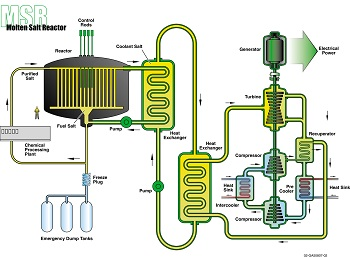
\includegraphics[width=0.8\textwidth]{gifmsr}
\caption{An MSR as envisioned by Gen-IV Forum.}
\label{fig:gifmsr}
\end{figure}

Currently, no widely accepted nuclear reactor analysis code can easily support drifting delayed neutron precursors. This phenomenon is nearly unique to molten salt reactors. Delayed neutron precursors are vital to reactor control, as shown by \cite[Ch. 6]{duderstadt_nuclear_1976}. The fission process leaves behind a small amount of delayed neutrons, typically emitting around 6 out of every 1000 new neutrons with a significant time delay. The effect is illustrated in Figure 2.

\begin{figure}
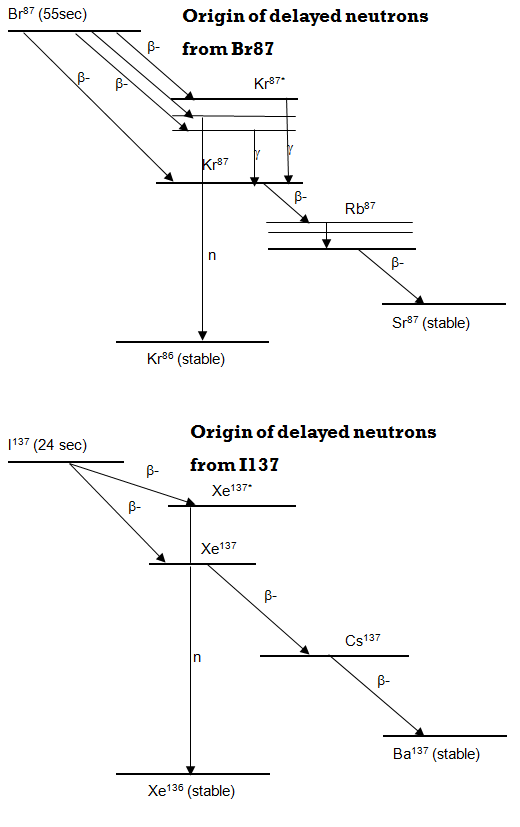
\includegraphics[width=0.8\textwidth]{dnp}
\caption{Examples of delayed neutron emitters.}
\label{fig:dnps}
\end{figure}

	As a result of the fissioning material drifting in a salt flow, delayed neutron precursors from freshly split atoms also move in salt flow. This leads to coupling between the neutron transport equation which governs the distribution of neutrons in a reactor to the Navier-Stokes equations, which govern fluid rheology and transport in the reactor. A more in-depth look at these equations will be covered in the methodology.

\cite{aufiero_calculating_2014} has made calculations with coupled neutronics to thermal-hydraulics, but in a molten
salt fast reactor. This study seeks to explore the same coupling, but in a thermal rather than fast
neutron spectrum. The only molten salt reactor ever built was the molten salt reactor experiment experiment (MSRE) documented in \cite{robertson_msre}. The MSRE was designed to be a small, thermal, low-power reactor to verify basic chemistry and neutron physics of the concept. This experiment yielded data which this project’s code can attempt to match. Possibly most important of all, thermal reactors can be built to be much smaller than fast reactor, easing the economic troubles of building large nuclear power plants. All of these reasons call for a need to develop versatile software accessible to those with a desire to bring a thermal MSR to market.
	Software was developed using sustainable, open principles to simulate both steady-state and transient behavior. Steady-state analysis was  performed using the Monte Carlo technique to solve the neutron transport equation (NTE) in the Serpent 2 code described in \cite{serp}. Transient analysis was simulated using a diffusion approximation to the NTE coupled to the incompressible Navier-Stokes equations. The resulting transient equations are solved with the open-source code described in \cite{moltres} called Moltres.

	\cite{duderstadt_nuclear_1976} covers the relevant reactor physics, including an introduction to diffusion theory and its appropriate modeling consideration. \cite{gaston_moose:_2009} gives an excellent example at the state of the art concerning multiphysics simulations of molten salt reactors. In order to efficiently write versatile, reproducible, and reusable code, this project implements the Multiphysics Object Oriented Simulation Environment Framework, or MOOSE Framework for short. \cite{aufiero_calculating_2014} describes the general philosophy and features of MOOSE. In order to use MOOSE, one must become familiar with the C++ programming language. \cite{schildt_c++:_2003} overviews C++.
    
The proposed project begins simulating simple problems representative of interesting physics exhibited by MSRs in the MOOSE framework. Next, more detailed physics simulations will be carried out in order to virtually replicate results from ORNL's MSRE. \cite{robertson_msre} cites several ORNL technical reports, each with experimental physics data. The experimental data will be used to confirm validity of the numerical models we seek to develop. Once ORNL experimental data can be replicated successfully, the aforementioned MOOSE models can be scaled to Blue Waters in order to investigate new physics including losses of cooling ability and sudden salt channel blockage.

All of the interesting physics in nuclear reactors results from the intense neutron field. Neutrons move about the reactor and split atoms, generating heat. The neutrons' overall average momenta and positions can be described approximately as a continuum, very much like Boltzmann's theory of gases detailed in \cite{boltzmann_lectures_2011}. The governing equation for neutron transport is:

% NTE
\begin{equation}
      \begin{aligned}
          \frac{1}{v(E)} \pd{\psi}{t} + \hat{\Omega}\cdot \nabla \psi + {\Sigma_t} \psi =&
          \frac{\chi_p(E)}{4 \pi} \int_{0}^{\inf} \nu_p(E') {\Sigma_f} {\phi} dE' + 
          \sum_i \frac{\chi_d(E)}{4 \pi} \lambda _i C_i + \\
          & \int_{4\pi}  \int_{0}^{\inf} {\Sigma_s(E'\rightarrow E,\hat{\Omega}'\rightarrow \hat{\Omega})} \psi dE' d\hat{\Omega}\\
      \end{aligned}
\label{eq:nte}
\end{equation}

% table of variables
\linespread{1}
\begin{table}[h]
\caption{Variables used in Equation \ref{eq:nte}.}
\centering
\begin{tabular}{c|c}
Variable & Meaning \\
\hline
$v$ & neutron velocity \\
E & neutron energy \\
$\psi$ & angular neutron flux \\
$\hat{\Omega}$ & unit vector of neutron motion \\
$\Sigma_t$ & total neutron cross section \\
$\chi_p$ & energy distribution of prompt neutrons \\
$\nu_p$ & average number of produced prompt neutrons \\
$\Sigma_f$ & nuclear fission cross section \\
$\phi$ & $=\int_{4\pi} |\psi| d\hat{\Omega}$, scalar neutron flux \\
$\chi_d$ & average energy of delayed neutrons \\
$\lambda_i$ & decay constant of $i$th delayed neutron group \\
$C_i$ & concentration of $i$th delayed neutron group \\
$\Sigma_s(E'\rightarrow E,\hat{\Omega}'\rightarrow \hat{\Omega})$ & cross section to scatter from energy $E'$ to $E$, angle $\Omega'$ to $\Omega$ \\
\end{tabular}
\end{table}
\linespread{2}

Equation \ref{eq:nte}'s high dimensionality requires enormous computational power to come to a direct numerical solution. Notice that the neutron transport equation is a Boltzmann transport equation as described in \cite{boltzmann_lectures_2011}, with no nonlinear terms and a collision kernel that represents neutrons colliding with nuclei. The probability of this collision can be given in units of inverse length, called the macroscopic cross section and symbolized by $\Sigma$. These interaction probabilities become functions of temperature through the Doppler broadening effect documented in Ch. 2 of \cite{duderstadt_nuclear_1976}, where resonances in nuclear cross sections become effectively broader on a plot of $\Sigma$ versus neutron energy due to the relative thermal motion of nuclei to incoming neutrons. Doppler broadening coupled with advection of delayed neutron precursors implies a tightly coupled physics problem between fluid flow, heat conduction, and neutron diffusion physics. The code Serpent 2 solves exclusively neutron transport using the Monte Carlo method, which traces individual neutrons through reactor geometry, binning their coordinates in the problem phase space in order to come to an extremely high fidelity solution. The Monte Carlo method is especially statistically efficient for solving neutron transport of regions of high neutron flux, like in a reactor. Knowledge of the neutron flux distribution over space and energy in the reactor allows determination of multigroup constants. Multigroup constants can be used in a different equation that approximates neutron transport as in Equation \ref{eq:nte}. The neutron diffusion equation for each group $g$ is:

% multigroup diffusion
\begin{equation}                \frac{1}{v_g}\frac{\partial {\phi}_g}{\partial t}   = \nabla \cdot D_g
                \nabla {\phi}_g +
                \sum_{g \ne g'}^G
                {\Sigma_{g'\rightarrow g}^s} {\phi}_{g'} + \chi_g^p \sum_{g' = 1}^G (1 -
                \beta) \nu {\Sigma_{g'}^f} {\phi}_{g'} + \chi_g^d \sum_i^I 
                \lambda_i {C_i} - {\Sigma_g^r} {\phi_g}
\label{eq:diff}
\end{equation}

\linespread{1}
\begin{table}
\caption{Variables used in multigroup diffusion, Equation \ref{eq:diff}.}
\label{tab:diffvar}
\centering
\begin{tabular}{c|c}
Variable & Meaning \\
\hline
$t      $    & \mbox{time} \\
$D_g    $    & \mbox{Diffusion coefficient for neutrons in group g} \\
$\Sigma_g^r$ & \mbox{macroscopic cross-section for removal of neutrons
from group g} \\
$\Sigma_{g'\rightarrow g}^s$ & \mbox{macroscopic cross-section of
scattering from g' to g} \\
$\chi_g^p$   & \mbox{prompt fission spectrum, neutrons in group g} \\
$G$          & \mbox{number of discrete groups, g} \\
$\nu$        & \mbox{number of neutrons produced per fission} \\
$\Sigma_g^f$ & \mbox{macroscopic cross section for fission due to neutrons in group g} \\
$\chi_g^d$   & \mbox{delayed fission spectrum, neutrons in group g} \\
$I $         & \mbox{number of delayed neutron precursor groups} \\
$\beta $     & \mbox{delayed neutron fraction}\\
$\lambda_i $ & \mbox{average decay constant of delayed neutron precursors
in precursor group i} \\
$C_i $       & \mbox{concentration of delayed neutron precursors in precursor
group i} .

\end{tabular}
\end{table}
\linespread{2}
All variables from Equation \ref{eq:diff} are described in Table \ref{tab:diffvar}. Notably, the diffusion equations reduce the neutron transport equation from a seven-dimensional problem into a system of four-dimensional problems. For code development, the problem is only solved in two dimensions. The problem can be scaled to hundreds of CPU cores on Blue Waters using the MOOSE framework. These large-scale simulations can provide knowledge on molten salt nuclear reactor behavior during accident events.

\subsection{Software}
This work will extend Moltres, an application within the MOOSE framework ecosystem. The MOOSE framework \cite{gaston_moose:_2009} allows scientists and engineers to easily implement advanced finite element methods such as discontinuous Galerkin or use niche basis functions like Hermite polynomials. The finite element method’s explanation is much out of the scope of this paper. \cite{aufiero_calculating_2014} explored the use of Monte Carlo to solve neutronics in a transient, so this paper seeks to explore the results produced by finite elements with deterministic (i.e. not Monte Carlo) neutronics. The neutron transport equation’s diffusion approximation will be solved using an approach coupling through both the temperature and density variables by generating group constants as functions of both temperature and density. Group constants are generated in Serpent following the method described in \cite{fridman_use_2011}.

	Code development will happen through git, particularly in the \url{github.com/arfc/moltres} repository \cite{moltres}. Serpent 2 input can be found at \url{github.com/gridley/msr-neutronics}. Some work has already been done in regards of simulating the reactor primary salt loop by coupling a postprocessor which takes an average across a mesh surface, into the reactor inlet. This allows the periodic advection of delayed neutron precursors, mass, and energy to be simulated.

A preliminary rendering of a cube-shaped reactor in steady-state is found in Figure \ref{fig:cubefig}. The simulation used all currently implemented neutron diffusion kernels, and uniform advection of heat and delayed neutron precursors in the +z direction.

\begin{figure}[ht]
\centering
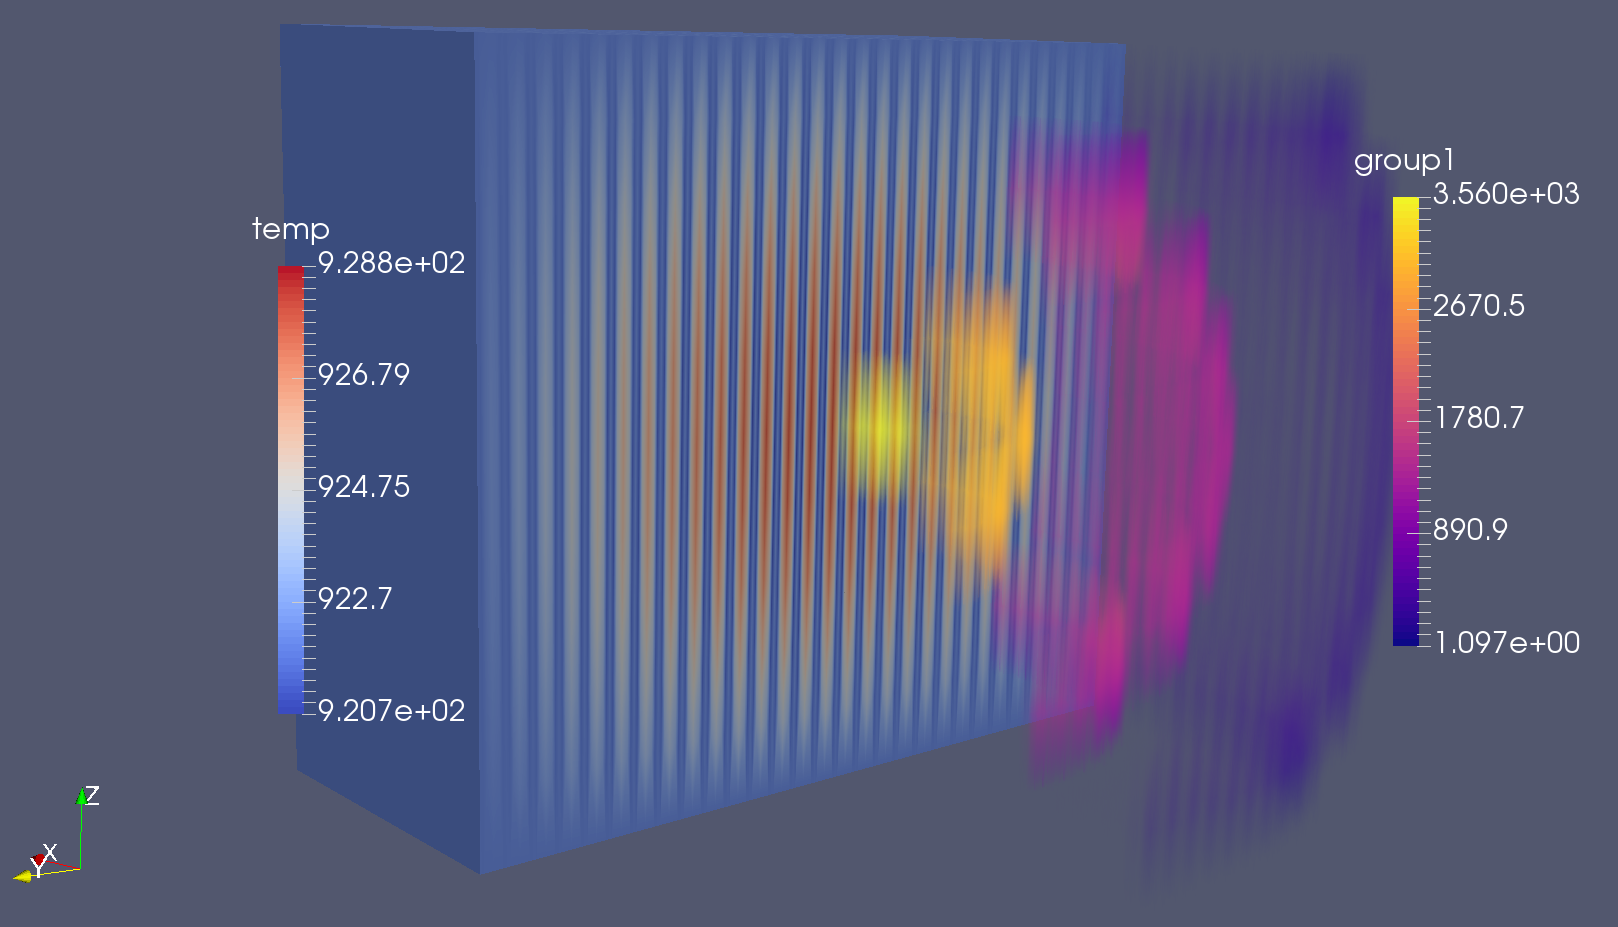
\includegraphics[width=0.8\textwidth]{cuboidal.png}
\caption{Preliminary simulation of coupled reactor fluxes and temperatures. Salt fraction matches ORNL MSRE value of 0.225.}
\label{fig:cubefig}
\end{figure}

\section{Methodology}

Three different types of reactor transient are simulated. First, a loss of core cooling through the primary heat exchanger is modeled. Next a loss of fuel pumping is simulated. Lastly a control rod removal transient is simulated. In order to run transient simulations efficiently, group constants for the reactor must first be generated. 

\subsection{Group Constants}
Typical reactor neutronic analysis makes use of the "two step method", where first a detailed code solves neutron transport using less approximate solutions to Equation \ref{eq:nte} such as fine energy group $S_N$ as in NEWT from the SCALE package \cite{kim_unstructured_2011} or continuous energy Monte Carlo as in Serpent \cite{serp}. Neutron cross sections depend on temperature significantly due to the previously described Doppler broadening, implying that cross sections must be generated as functions of temperature.

Typically, reactor cross sections get homogenized and subsequently condensed, as described in \cite{stammler_methods_1983} Ch. 1. 
For high fidelity neutronics simulation, cross sections are only condensed into a coarse group energy structure. In \cite{gentry} a coarse group energy structure was devised for high temperature graphite moderated, salt cooled reactors with embedded TRISO. The optimal group structure calculated here has two thermal, one resonance, and one fast group, evidencing the strongly upscattering nature of this reactor specie. \cite{gentry} refers to the optimal structure as "option 1". We choose this group structure for use in salt fueled reactors moderated by graphite since neutron energy spectra can be expected to be similar in nature; both reactors operate at high temperature and have roughly the same set of materials in the core.

Multigroup cross sections are defined as:

\begin{equation}
\Sigma_g = \frac{\int_{\Omega_g} \phi(E) \Sigma_{fine}(E) dE}{\int_{\Omega_g} \Sigma_{fine} dE}
\end{equation}

Where $g$ is the energy group, $\Omega_g$ is domain of energies in group $g$, $\phi(E)$ is the flux, and $\Sigma$ and $\Sigma_{fine}$ represent cross sections for respectively the condensed and fine nuclear data. Clearly this implies that group constants depend on just fine nuclear data and the fine energy group flux solution. In the MSRE, control rod insertion will preferentially absorb thermal neutrons, since the Gd$_2$O$_3$ rings exhibit strong thermal absorption with relatively weak resonance absorption. Thermal neutrons have a small mean free path. Thus, control rod influence on reactor spectrum should be small away from the rods, but still greatly reduce reactor $k$ eigenvalue since the chain reaction cannot be sustained. Upon taking this in consideration, all reactor simulations hereafter only utilize group constants which are functions of temperature, although the constants for control rod position are indeed available in the Moltres github repository.

The ORNL MSRE was modeled as per original documentation in \cite{robertson_msre}. Salt channel geometry was modeled exactly. Control rod guide tubes were explicitly modeled. The experiment tube was modeled as a cylinder filled with graphite due to its geometric complexity. The resulting geometry can be found in Figure \ref{fig:msreGeometry}. The model geometry can be compared to the experiment's actual geometry in Figure \ref{fig:actualMSRE}. All Serpent 2 input can be found at \url{https://github.com/gridley/msr-neutronics/tree/MSRE/MSRE}. 

\begin{figure}[ht]
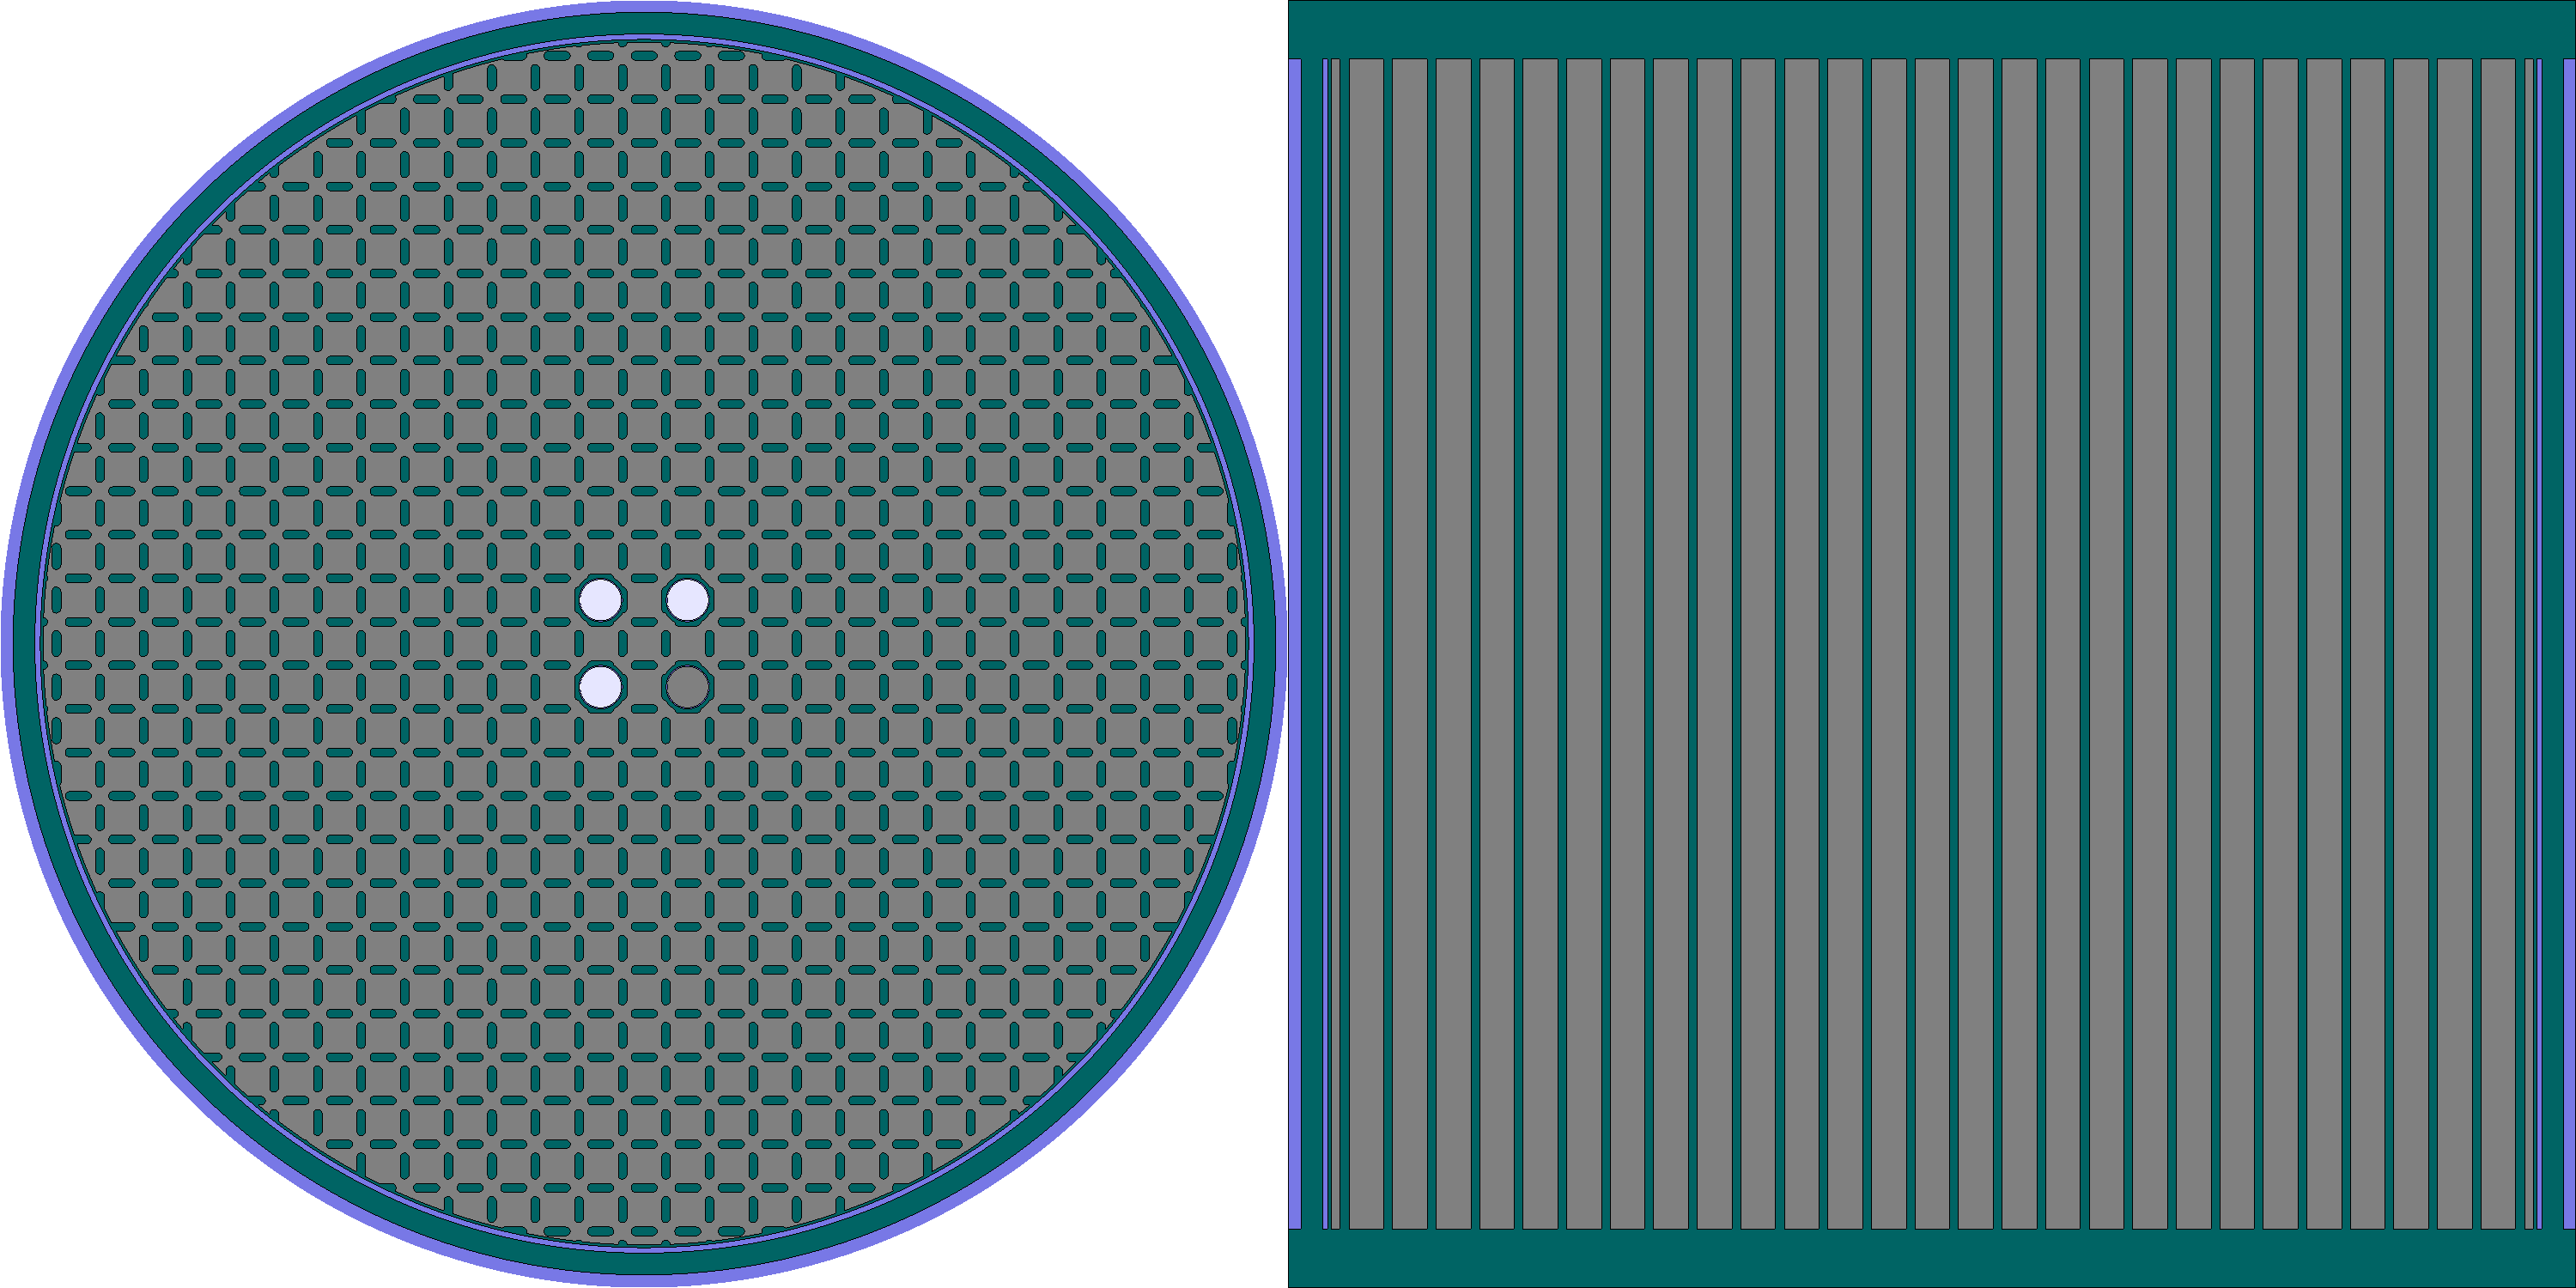
\includegraphics[width=\textwidth]{msreSerpGeom.png}
\caption{Left: radial plane cut of MSRE geometry. Right: RZ plane cut. MSRE neutronics geometry for Serpent. Graphite is grey, INOR-8 alloy is purple, and salt is teal.}
\label{fig:msreGeometry}
\end{figure}

\begin{figure}[ht]
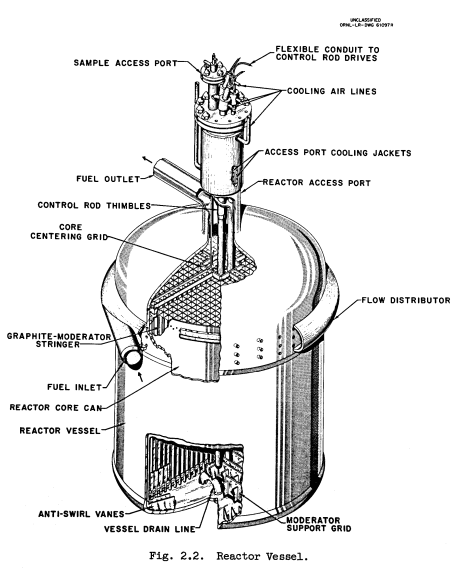
\includegraphics[width=\textwidth]{actualMSRE.png}
\caption{An MSRE final design sketch from \cite{robertson_msre} for comparison to Figure \ref{fig:msreGeometry}.}
\label{fig:actualMSRE}
\end{figure}

\subsection{MOOSE Model}
For MOOSE transient calculations, calculations were done on a simple 2D mesh that mimics the physics of the MSRE. Salt fraction was kept the same, and the problem was solved in RZ coordinates. More intuitively, this means that the problem was solved on an equivalent reactor made of concentric rings of graphite and fuel salt.
The \texttt{gmsh} \cite{gmsh} tool was used to generate the file containing all element node locations and connectivity information.
Figure \ref{fig:msremesh} illustrates the computational domain produced by \texttt{gmsh} that models the MSRE.

\begin{figure}[ht]
\centering
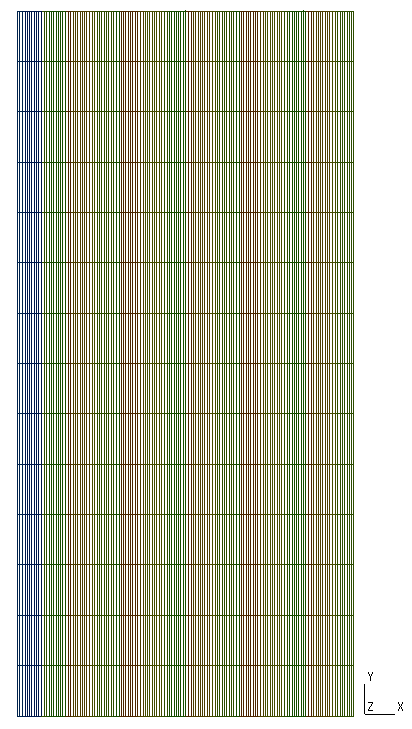
\includegraphics[width=0.4\textwidth]{msre2DMesh}
\caption{Mesh used to model MSRE produced by \texttt{gmsh}. Blue is a control rod region, green is moderator, and yellow is fuel. Y is the axial coordinate here and X is the radial.}
\label{fig:msremesh}
\end{figure}

\begin{figure}
\centering
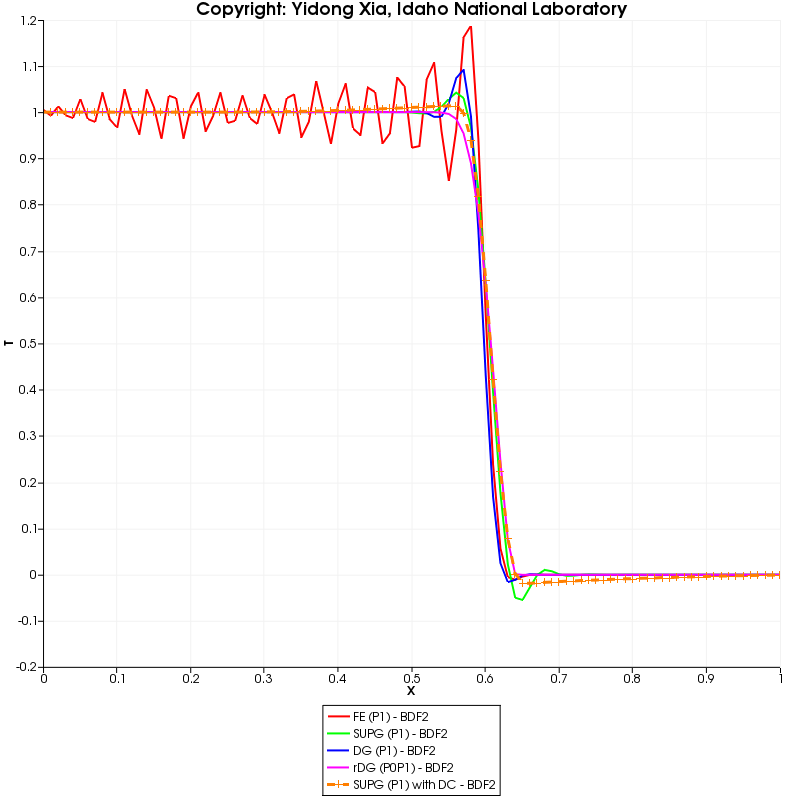
\includegraphics[width=0.5\textwidth]{xiaDG}
\caption{Comparison of continuous Galerkin (CG) and discontinous (DG). DG is markedly more stable. Credit Yidong Xia.}
\label{fig:DGISKEWL}
\end{figure}

Neutronics get solved in multigroup diffusion using a two group structure using Galerkin FEM. Precursor decay, production, and advection are solved using discontinous Galerkin since advection with no diffusive character can be far more unstable than continuous Galerkin, as depicted by Figure \ref{fig:DGISKEWL}. Heat transfer is solved using continuous Galerkin. No thermalhydraulic models are employed since the flow in the MSRE is laminar: calculating the Reynolds number from \cite{robertson_msre} yields Re$=858$, much lower than the turbulent flow limit of Re=$2200$ as discussed in \cite{schmidt_introduction_1993}. As a result, continuous temperature at the graphite/fuel boundary correctly resolves the temperature variable.

\subsection{Control Rods}

To simulate control rod movement in molten salt reactors, a new material was added to Moltres \cite{moltres} called \texttt{RoddedMaterial}. This new material returns strongly neutron absorbing material properties below the control rod height, and user-defined material properties below the rod height. The rod height can be dynamically changed through the MOOSE controls module. The ORNL MSRE's control rods moved in response to transient effects, so this control rod position data versus time in transient would be used to match experiment. Thus, \texttt{RoddedMaterial} will be useful for future studies. An example of the new feature in action can be seen in Figure \ref{fig:controlrod}.

\begin{figure}
\centering
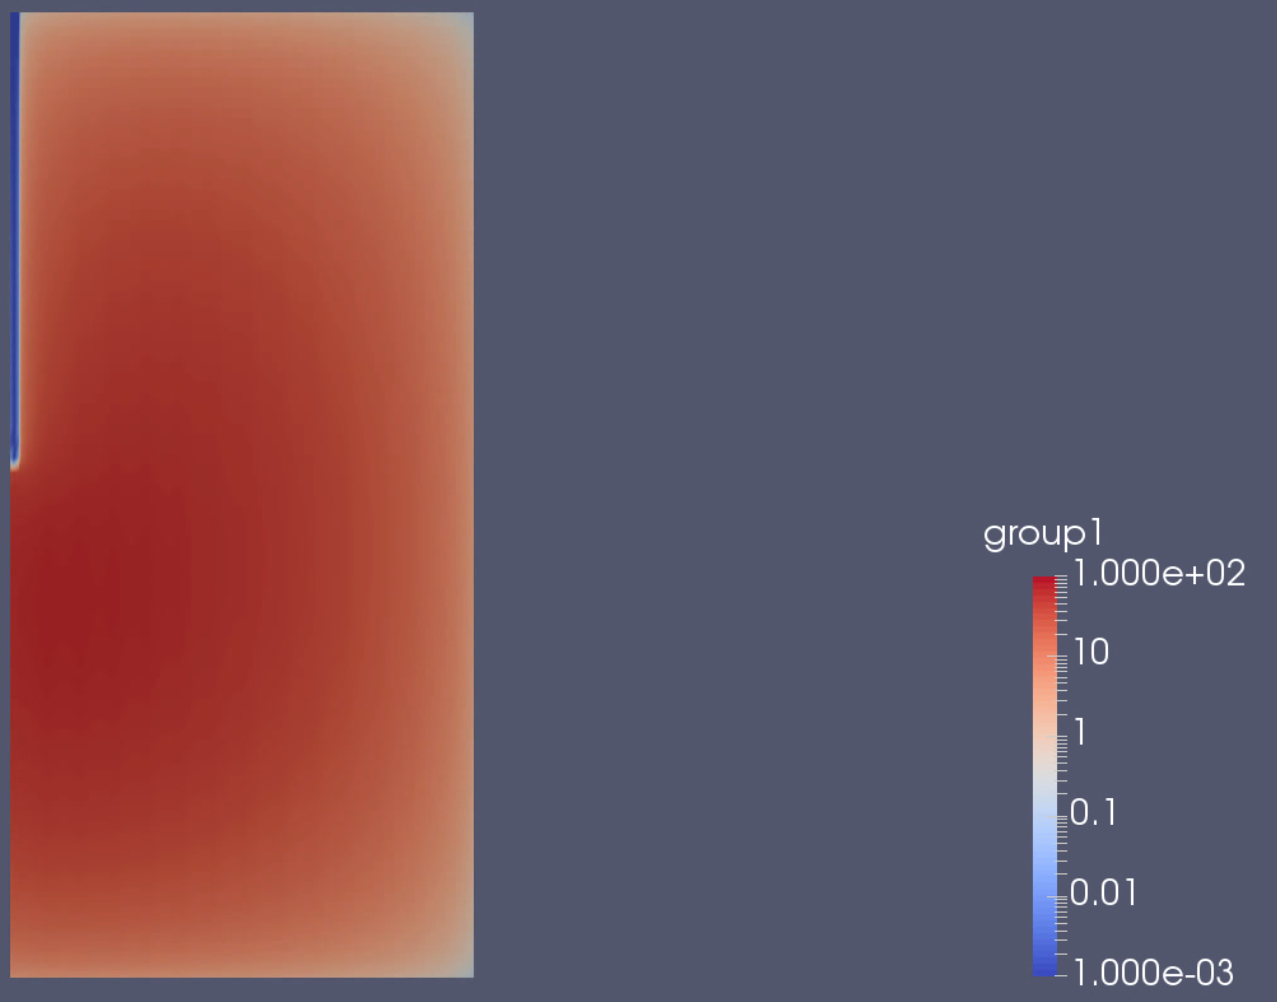
\includegraphics[width=0.7\textwidth]{controlrod}
\caption{Clearly visible influence of control rod on reactor power profile.}
\label{fig:controlrod}
\end{figure}

\subsection{Loss of Cooling Accidents}

The ability to simulate loss of cooling accidents was added to the Moltres code. The reactor primary fuel loop was modeled as a separate one-dimensional problem using a MOOSE MultiApp. Transport in the primary loop was solved using discontinuous Galerking and a Dirac delta function normalized to remove the correct amount of power. The piece of code in Moltres is called \texttt{DiracHX}. It was found that using a Dirac delta usually led to a different amount of heat being removed from the system than expected. Instead, a MOOSE InterfaceKernel called \texttt{InterfaceHX} was implemented that successfully removed the correct amount of heat.

The heat removal rate was made controllable through the MOOSE controls module. In doing so, the heat removal rate can be changed according to any user-specified parsed function. Not only loss of cooling could be simulated; power change maneuvers could be simulated as well.

\subsection{Loss of Flow Accidents}

Simulating a loss of fuel flow accident requires that the salt velocity variable be changed through the MOOSE controls module. In the past, Moltres \cite{moltres} has relied upon its \texttt{Squirrel} module to provide dicontinuous Galerkin transport kernels. Many of these kernels and DG boundary conditions only accept constant velocity variable inputs. The code was appropriately modified so that velocity can be set through the MOOSE controls module. For all loss of flow transients, the same approach of modeling the primary loop by a one-dimensional problem and InterfaceKernel was taken.

\section{Results}

\subsection{Control Rod Withdrawal}

\subsection{Loss of Cooling}

\subsection{Loss of Flow}

\section{Discussion}



\section{Conclusion}
Group constants for the ORNL Molten Salt Reactor experiment were generated as functions of fuel temperature, moderator temperature, and control rod position. Reactor simulations looking up group constants as a function of control rod position never came to realization since other tools required for a reactor simulation had to be developed beforehand.

For realistic transients simulations of MSRs, decay heat simulation should be added to Moltres. This will usually be around 6\% of the average reactor power. Standards to be implemented can be found in \cite{decay}.

Natural convection will dominate MSR steady temperature in the shutdown state, provided that no forced convection is provided. Some ability to model natural convection has been added to Moltres, but as of yet simulating reactors with natural convection is untested.

Radiative heat transfer will likely largely influence the reactor vessel temperature at all hot operating states. In fact, these reactors' pipes will be red-hot in operation, as evidenced by the MSRE heat sink to the atmosphere from \cite{robertson_msre}. Radiative heat transfer models like from \cite{schmidt_introduction_1993} should be implemented in Moltres.

In loss of flow transients, the influence of subcooling on due to slowing flow may cause power to rise soon after losing power to th pump for some flywheel size. This effect should be investigated and plotted.

\FloatBarrier

\bibliographystyle{plain}
\bibliography{bibli}

\end{document}
